\chapter*{Introduction}
\addcontentsline{toc}{chapter}{Introduction}
\markboth{Introduction}{Introduction}
\index{Material Point Method!overview}
\index{Material Point Method!history}
\index{applications}
\index{GEOS-MPM!applications}
\index{GEOS!main repository}
\index{GEOS!documentation}
\index{GEOS-MPM!lightweight branch}

The Material Point Method (MPM) is a hybrid Eulerian--Lagrangian discretization for continuum mechanics.  Material is represented by Lagrangian particles that carry mass, position, volume, velocity, stress, deformation gradient, damage, temperature, and other history-dependent internal variables.  A background grid is used only as a computational scratchpad for the momentum balance.  In a typical explicit step, particle mass, momentum, stress divergence, and body forces are mapped to grid nodes; nodal accelerations and velocities are advanced subject to contact and boundary conditions; particle kinematics and material state are updated; and the grid is reset before the next step.  This organization retains the history-tracking advantages of a Lagrangian method while avoiding the mesh entanglement that limits conventional finite elements in very large deformation, evolving contact, fracture, fragmentation, and granular-flow problems.

\begin{center}
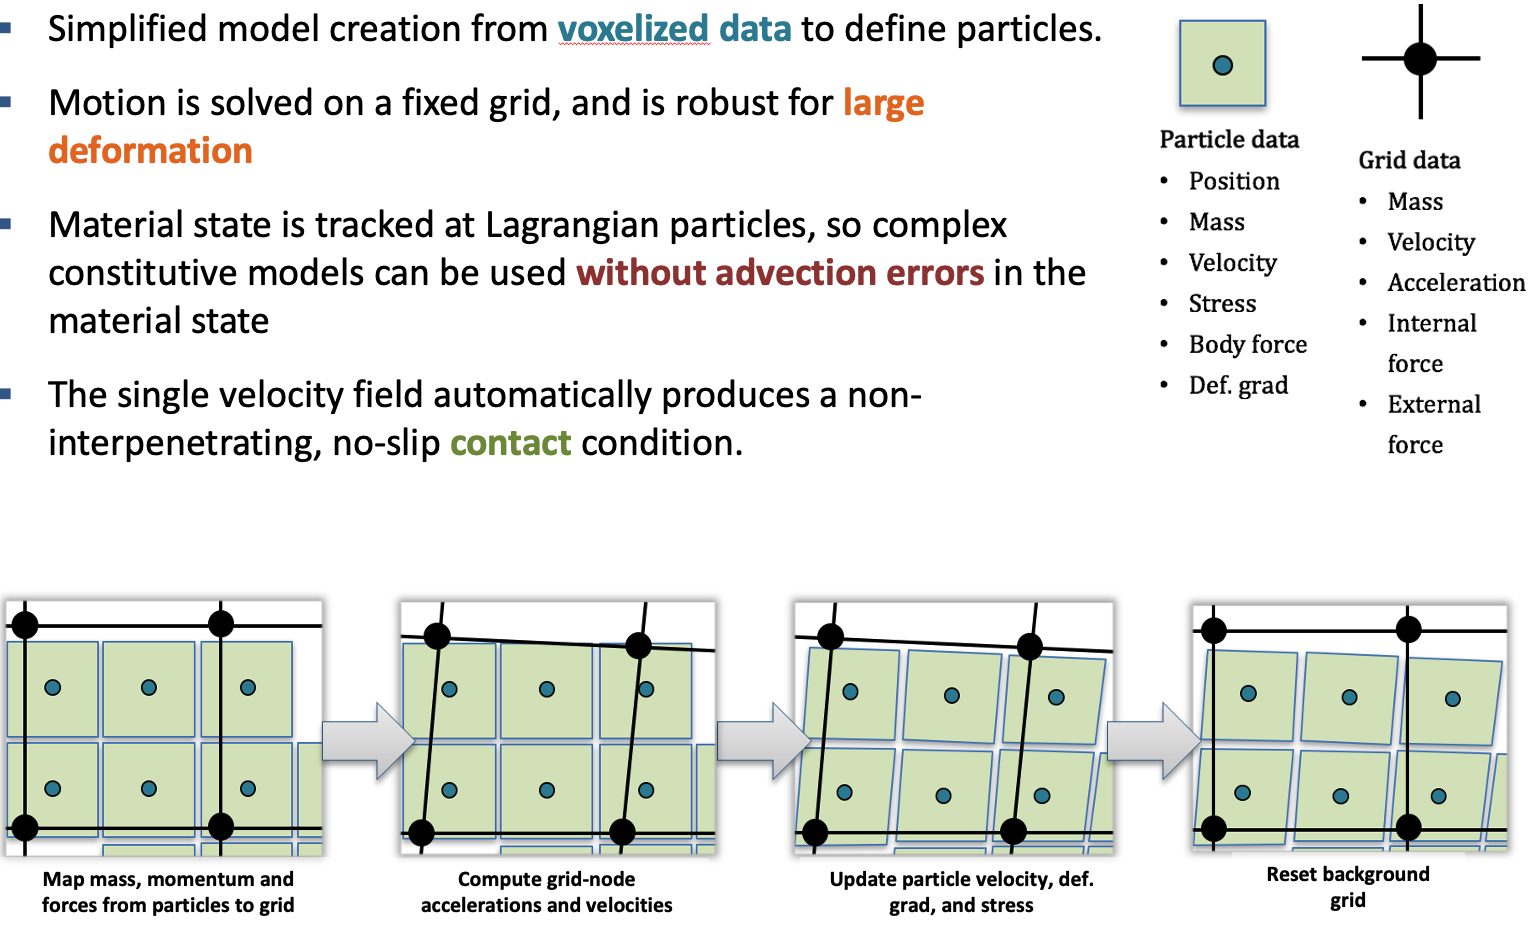
\includegraphics[width=0.95\linewidth]{figures/mpm_overview_diagram.png}
\captionof*{figure}{High-level MPM data model and update cycle.  Particles carry material state, while the background grid supplies a temporary computational frame for mass, momentum, force, acceleration, boundary-condition, and contact updates.}
\end{center}

\section*{Relationship to the main GEOS project}
\phantomsection
\addcontentsline{toc}{section}{Relationship to the main GEOS project}
The main GEOS open-source project is hosted at the GEOS-DEV repository, \url{https://github.com/GEOS-DEV/GEOS}, and its public user/developer documentation is available through the GEOS documentation site, \url{https://geosx-geosx.readthedocs-hosted.com/en/latest/}.  GEOS-MPM is developed in the same software ecosystem, but this manual is written for the MPM-focused branch rather than for the current public release/develop branch of the main GEOS project.  At the time this manual was prepared, the main GEOS release and develop branches contain only an early MPM solver snapshot relative to the code documented here.

The MPM branch intentionally reuses the pieces of GEOS that are valuable for large-deformation particle mechanics: the XML/object catalog and data-repository model, the GEOS internal Cartesian mesh generator, MPI domain decomposition and ghosting infrastructure, event scheduling, restart/output utilities, constitutive-model registration, unit/integrated-test conventions, and the CMake-based build system.  Conversely, a lightweight MPM build does not need many finite-element, finite-volume, reservoir-flow, well, compositional-fluid, and solver-stack components required by the GEOS flow, fracture, and poromechanics applications.  This branch is therefore maintained to support MPM-specific build tools that remove third-party libraries not required by MPM, while also providing detailed MPM and ParticleFileWriter documentation that would be too specialized for most finite-element/finite-volume GEOS users.

\section*{Brief MPM history}
\phantomsection
\addcontentsline{toc}{section}{Brief MPM history}
The MPM descends from particle-in-cell (PIC) and FLIP ideas developed for computational fluid dynamics, in which particles carry advected state and a grid is used to solve the equations of motion \cite{harlow1964pic,brackbill1988flip}.  Sulsky, Chen, and Schreyer introduced the modern MPM formulation for history-dependent solid materials, and Sulsky, Zhou, and Schreyer established its solid-mechanics interpretation for large-deformation calculations \cite{sulsky1994history,sulsky1995solid}.  Subsequent developments reduced grid-cell-crossing and quadrature error, generalized particle-to-grid interpolation, and improved contact and fracture treatment.  Examples important to GEOS-MPM include GIMP \cite{bardenhagen2004gimp}, convected particle domain interpolation (CPDI) and CPDI2 \cite{sadeghirad2011cpdi,sadeghirad2013cpdi2}, Bardenhagen--Guilkey multi-field contact \cite{bardenhagen2001contact}, Nairn's explicit-crack and later contact/update algorithms \cite{nairn2003cramp,nairn2020contact}, Homel--Herbold damage-field-gradient partitioning \cite{homel2016dfg}, and Crook--Homel cohesive-zone treatment for large deformation and damage \cite{crook2025cohesive}.

GEOS-MPM follows this lineage but is organized around GEOS-style input generation and multiphysics extensibility.  The code emphasizes voxelized or image-derived geometries, large-deformation solid dynamics, frictional contact, continuum damage, cohesive fracture, CPDI-domain treatments, and verification through generated particle files and repeatable simulation suites.

\section*{Application scope}
\phantomsection
\addcontentsline{toc}{section}{Application scope}
\index{applications!large deformation}
\index{applications!fracture}
\index{applications!granular materials}
\index{applications!voxelized data}
MPM and MPM-derived methods have been used across several application classes that motivate GEOS-MPM features:
\begin{itemize}[leftmargin=*]
\item \textbf{Porous and heterogeneous geomaterials.}  Image-derived and mesoscale material descriptions can represent pores, inclusions, grains, weak interfaces, and material heterogeneity directly by particles or particle-associated state variables \cite{homel2017mesoscalevalidation,homel2017porous}.
\item \textbf{Large deformation with CPDI domain scaling.}  CPDI domain scaling controls the onset of numerical fracture in massively deforming, parallel MPM calculations, a key issue for compaction, indentation, fracture, and high-distortion solid-mechanics simulations \cite{homel2016domaindef}.
\item \textbf{Fracture and frictional self-contact.}  Damage-field-gradient partitioning creates local kinematic enrichment without predefining every contact pair.  The method supports dynamic crack propagation, self-contact, frictional sliding, granular flow, porous compaction, fragmentation, and comminution of brittle materials \cite{homel2016dfg}.
\item \textbf{Mesoscale porous and heterogeneous materials.}  DFG-based MPM supports simulations aimed at mesh-independent particle-size distributions in comminution and fragmentation problems, as well as damage evolution in heterogeneous solids \cite{homel2017porous}.
\item \textbf{Large-deformation cohesive fracture and exact-surface contact.}  The Crook--Homel cohesive-zone formulation adds explicit surface geometry, cohesive tractions, and exact-surface contact data paths for problems in which curved interfaces and under-resolved binder or interface layers are important \cite{crook2025cohesive}.
\item \textbf{Image-based mesoscale damage in concrete and related composites.}  Mesoscale modeling together with X-ray computed micro-tomography motivates the voxelized-data and image-based mesostructure workflows supported by PFW \cite{homel2022uhpc}.
\end{itemize}

\begin{figure}[htbp]
\centering
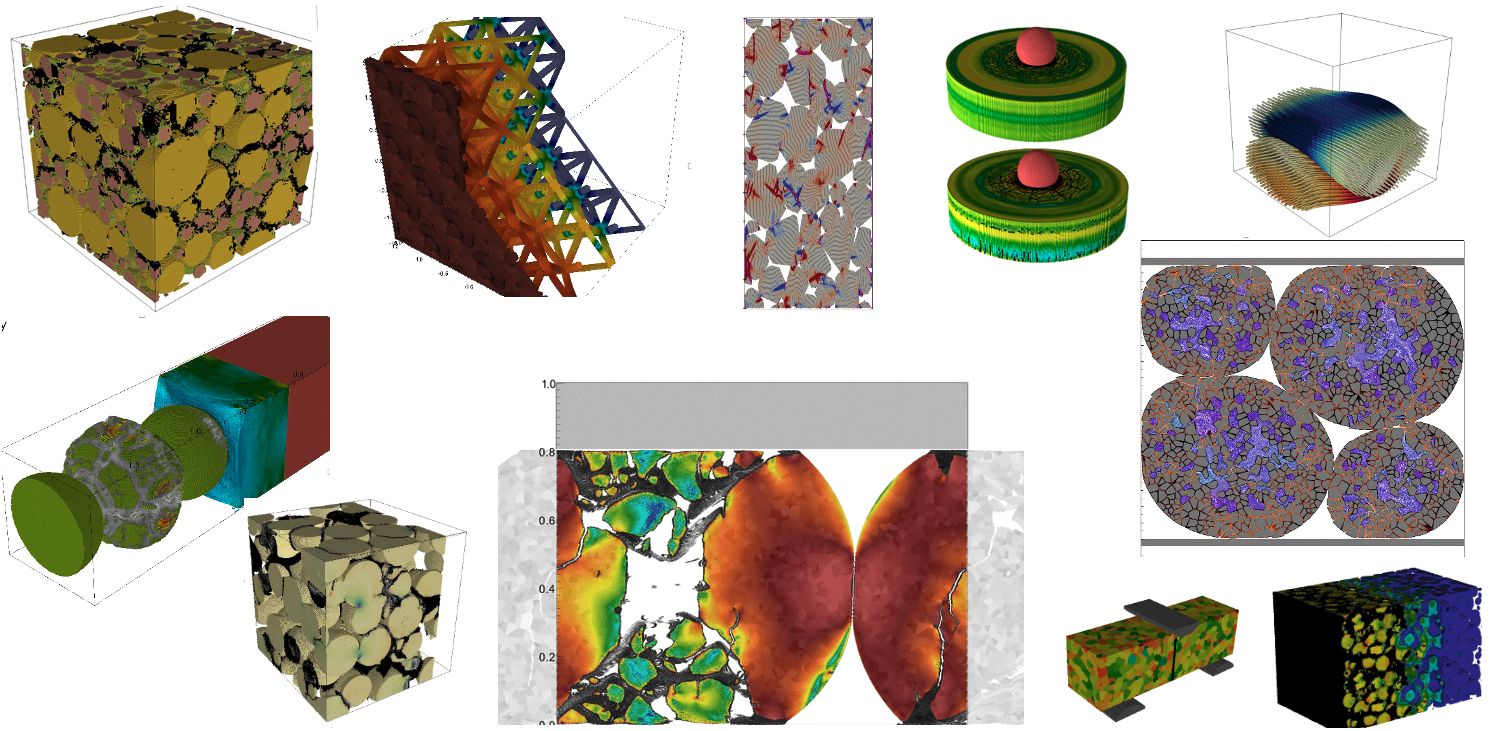
\includegraphics[width=0.98\linewidth]{figures/mpm_applications_composite.png}
\caption{Examples of the type of large-deformation solid-mechanics simulations for which the Material Point Method is well suited: voxelized and image-derived mesostructures, heterogeneous compaction, fracture, contact, indentation, torsion, and coupled damage/flow of fragmented solids.}
\label{fig:mpm-applications-composite}
\end{figure}

This manual therefore treats GEOS-MPM as both a production code and a research platform: the same particle-grid structure supports classical MPM, CPDI and B-spline mapping, PIC/FLIP/XPIC/FMPM update options, multi-field and DFG contact, cohesive-zone surfaces, and robustness controls for deletion, deformation-gradient reset, and particle splitting.
